% 2013-03-04_geo.tex
% 2013-03_03 dmontaner@cipf.es
% Master en Bioinformatica UV
% Nociones básicas de bioinformática y genómica

%% INTRODUCTION TO GEO 

\documentclass{beamer}
\usepackage[utf8]{inputenc}
%\usepackage[spanish]{babel}
%\usepackage[spanish,english]{babel}
\usepackage[english]{babel}

\hypersetup{colorlinks=true, citecolor=black, filecolor=black, linkcolor=blue, urlcolor=blue} %color de los links %\usepackage{hyperref} va incluido
\setbeamertemplate{frametitle}[default][center]
\setbeamertemplate{itemize items}[ball]

\graphicspath{{plots/}}

%\usepackage{enumitem}
%\usepackage{mdwlist}
%%%%%%%%%%%%%%%%%%%%%%%%%%%%%%%%%%%%%%%%%%%%%%%%%%%%%%%%%%%%%%%%%%%%%%%%%%%%%%%%

\title{GEO}
\date{11 March 2013}

\subtitle{Gene Expression Omnibus}
\author{David Montaner \\ 
  %\href{http://www.dmontaner.com}{http://bioinfo.cipf.es/dmontaner} \\ 
  \href{http://www.dmontaner.es/materiales}{www.dmontaner.es/materiales} \\ 
  %\href{mailto:dmontaner@cipf.es}{dmontaner@cipf.es}}
  dmontaner@cipf.es}


%%%%%%%%%%%%%%%%%%%%%%%%%%%%%%%%%%%%%%%%%%%%%%%%%%%%%%%%%%%%%%%%%%%%%%%%%%%%%%%%
%% DOCUMENTO %%%%%%%%%%%%%%%%%%%%%%%%%%%%%%%%%%%%%%%%%%%%%%%%%%%%%%%%%%%%%%%%%%%
%%%%%%%%%%%%%%%%%%%%%%%%%%%%%%%%%%%%%%%%%%%%%%%%%%%%%%%%%%%%%%%%%%%%%%%%%%%%%%%%
\begin{document}
\begin{frame}
  \maketitle
\end{frame}

%\begin{otherlanguage}{spanish}

%%%%%%%%%%%%%%%%%%%%%%%%%%%%%%%%%%%%%%%%%%%%%%%%%%%%%%%%%%%%%%%%%%%%%%%%%%%%%%%%
%% SLIDES empiezan aqui despues del titulo %%%%%%%%%%%%%%%%%%%%%%%%%%%%%%%%%%%%%
%%%%%%%%%%%%%%%%%%%%%%%%%%%%%%%%%%%%%%%%%%%%%%%%%%%%%%%%%%%%%%%%%%%%%%%%%%%%%%%%

%\setbeamerfont*{itemize/enumerate body}{size=\footnotesize}

\begin{frame}[allowframebreaks]
  \frametitle{Microarray Databases}

  \begin{itemize}
  \item GeneNetwork system: Open access standard arrays, exons arrays, and RNA-seq data for genetic analysis (eQTL studies) with analysis.
  \item UNC modENCODE Microarray database: Nimblegen customer 2.1 million array 6.
  \item UPSC-BASE: data generated by microarray analysis within Umeå Plant Science Centre (UPSC).
  \item UPenn RAD database: MIAME compliant public and private studies, associated with ArrayExpress.
  \item UNC Microarray database: provides the service for microarray data storage, retrieval, analysis, and visualization.

    \framebreak

  \item MUSC database: The database is a repository for DNA microarray data generated by MUSC investigators as well as researchers in the global research community.
  \item caArray at NCI: Cancer data, prepared for analysis on caBIG.
  \item ArrayTrack: ArrayTrack hosts both public and private data, including MAQC benchmark data, with integrated analysis tools.
  \item NCI mAdb: Hosts NCI data with integrated analysis and statistics tools.
  \item ImmGen database: Open access across all immune system cells; expression data, differential expression, coregulated clusters, regulation.

    \framebreak

  \item Genevestigator database: Gene expression search engine based on manually curated microarray data.
  \item \href{http://www.ncbi.nlm.nih.gov/geo/}{\textbf{Gene Expression Omnibus (GEO)}}: NCBI any curated MIAME compliant molecular abundance study.
  \item \textbf{ArrayExpress}: at EBI Any curated MIAME or MINSEQE compliant transcriptomics data.
  \item Stanford Microarray database: private and published microarray and molecule abundance database.
  \end{itemize}

  \bigskip
  %\vspace{20 mm}  
  %\center
  {\footnotesize Source: \url{http://en.wikipedia.org/wiki/Microarray_databases}}

\end{frame}

%%%%%%%%%%%%%%%%%%%%%%%%%%%%%%%%%%%%%%%%%%%%%%%%%%%%%%%%%%%%%%%%%%%%%%%%%%%%%%%%

\begin{frame}
  \frametitle{GEO}

  \textbf{Gene Expression Omnibus:} a public functional genomics data repository supporting MIAME-compliant data submissions. 
  Array and sequence-based data are accepted. Tools are provided to help users query and download experiments and curated gene expression profiles.

  \bigskip
  
  \textbf{MIAME:} Minimum Information About a Microarray Experiment)

  \bigskip

  \textit{Minimum information about a microarray experiment (MIAME)-toward standards for microarray data.}
  Brazma et. al (2001) 
  Nat Genet. 2001 Dec;29(4):365-71.
  PMID: 11726920 [PubMed - indexed for MEDLINE] 
  
\end{frame}

%%%%%%%%%%%%%%%%%%%%%%%%%%%%%%%%%%%%%%%%%%%%%%%%%%%%%%%%%%%%%%%%%%%%%%%%%%%%%%%%

\begin{frame}
  \frametitle{MIAME}
  
  % MIAME: Minimum Information About a Microarray Experiment

  \begin{itemize}
  \item The raw data for each hybridization (e.g., CEL or GPR files)
  \item The final normalized data for the set of hybridizations in the study (e.g. gene expression data matrix)
  \item The essential sample annotation (e.g., compound and dose in a dose response experiment, class)
  \item The experimental design including sample data relationships (e.g. technical and biological replicates)
  \item Sufficient annotation of the array (e.g. gene identifiers, genomic coordinates, probe oligonucleotide sequences)
  \item The essential laboratory and data processing protocols (e.g., what normalization method)
  \end{itemize}
  
\end{frame}

%%%%%%%%%%%%%%%%%%%%%%%%%%%%%%%%%%%%%%%%%%%%%%%%%%%%%%%%%%%%%%%%%%%%%%%%%%%%%%%%

\begin{frame}[allowframebreaks]
  \frametitle{Data Organization in GEO}

  Original data (submitted by researchers)

  \begin{itemize}
  \item \textbf{Platform} record: summary description of the array template. \\
    GEO accession number: \textbf{GPL}xxx
  \item \textbf{Sample} record: individual sample data (genomic, phenotypic, experimental \dots) \\
    GEO accession number: \textbf{GSM}xxx
  \item \textbf{Series} record: a group of related samples, usually from one experiment or study. \\
    GEO accession number \textbf{GSE}xxx.
  \end{itemize}
  
  \framebreak
  
  Curated data (organized by GEO)
  
  \begin{itemize}
  \item \textbf{DataSet} records: a curated collection of \textit{biologically and statistically comparable} samples
    reassembled by GEO staff form one or several series \\
    GEO accession number \textbf{GDS}xxx.  \\
    For them GEO has data display and analysis tools. 
  \item \textbf{Gene Profiles}: measurements for an individual gene across all Samples in a DataSet.
  \end{itemize}
      
\end{frame}

%%%%%%%%%%%%%%%%%%%%%%%%%%%%%%%%%%%%%%%%%%%%%%%%%%%%%%%%%%%%%%%%%%%%%%%%%%%%%%%%

\begin{frame}
  \frametitle{GEO Web Query}
  
  Query
  
  \begin{itemize}
  \item \href{http://www.ncbi.nlm.nih.gov/gds/}{DataSets}: Stores curated gene expression DataSets. \\
    Search example: \textit{melanoma}
  \item \href{http://www.ncbi.nlm.nih.gov/geoprofiles/}{Gene profiles}: Stores individual gene expression profiles from curated DataSets. \\
    Search example: \textit{melanoma}
  \item \href{http://www.ncbi.nlm.nih.gov/geo/query/acc.cgi}{\textbf{GEO accession}}: Searches GEO Accessions. \\ 
    Search example: \href{http://www.ncbi.nlm.nih.gov/geo/query/acc.cgi?acc=GSE37761}{\textit{GSE37761}}
  \end{itemize}

  \bigskip
  
  Browser: \textit{nicer interface; exports searches}

  \begin{itemize}
  \item \href{http://www.ncbi.nlm.nih.gov/sites/GDSbrowser}{DataSets} \\
    Search example: \textit{melanoma}
  \item \href{http://www.ncbi.nlm.nih.gov/geo/browse/}{GEO accession}: Platforms; Samples; Series \\
    Search example: \textit{melanoma}
  \end{itemize}

  %\bigskip

  \begin{center}
    \url{http://www.ncbi.nlm.nih.gov/geo/}
  \end{center}  

\end{frame}

%%%%%%%%%%%%%%%%%%%%%%%%%%%%%%%%%%%%%%%%%%%%%%%%%%%%%%%%%%%%%%%%%%%%%%%%%%%%%%%%

\begin{frame}
  \frametitle{GEO Web}
  
  \begin{center}
    %\includegraphics[scale=0.3]{} 
    \href{http://www.ncbi.nlm.nih.gov/geo/}{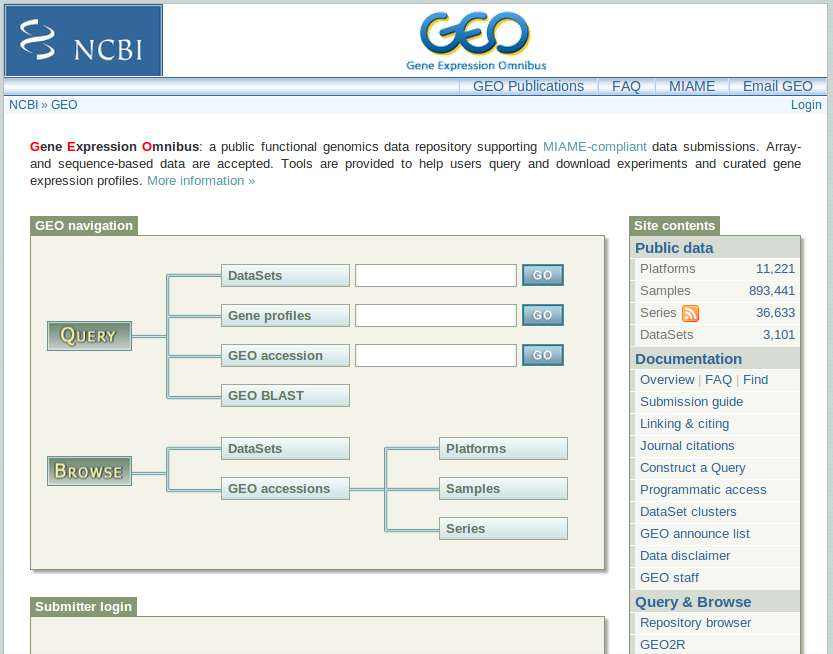
\includegraphics[width=\linewidth]{geo1}}
  \end{center}

\end{frame}

%%%%%%%%%%%%%%%%%%%%%%%%%%%%%%%%%%%%%%%%%%%%%%%%%%%%%%%%%%%%%%%%%%%%%%%%%%%%%%%%

\begin{frame}
  \frametitle{GEO at NCBI}
  
  \begin{center}
    %\includegraphics[scale=0.3]{} 
    \href{http://www.ncbi.nlm.nih.gov}{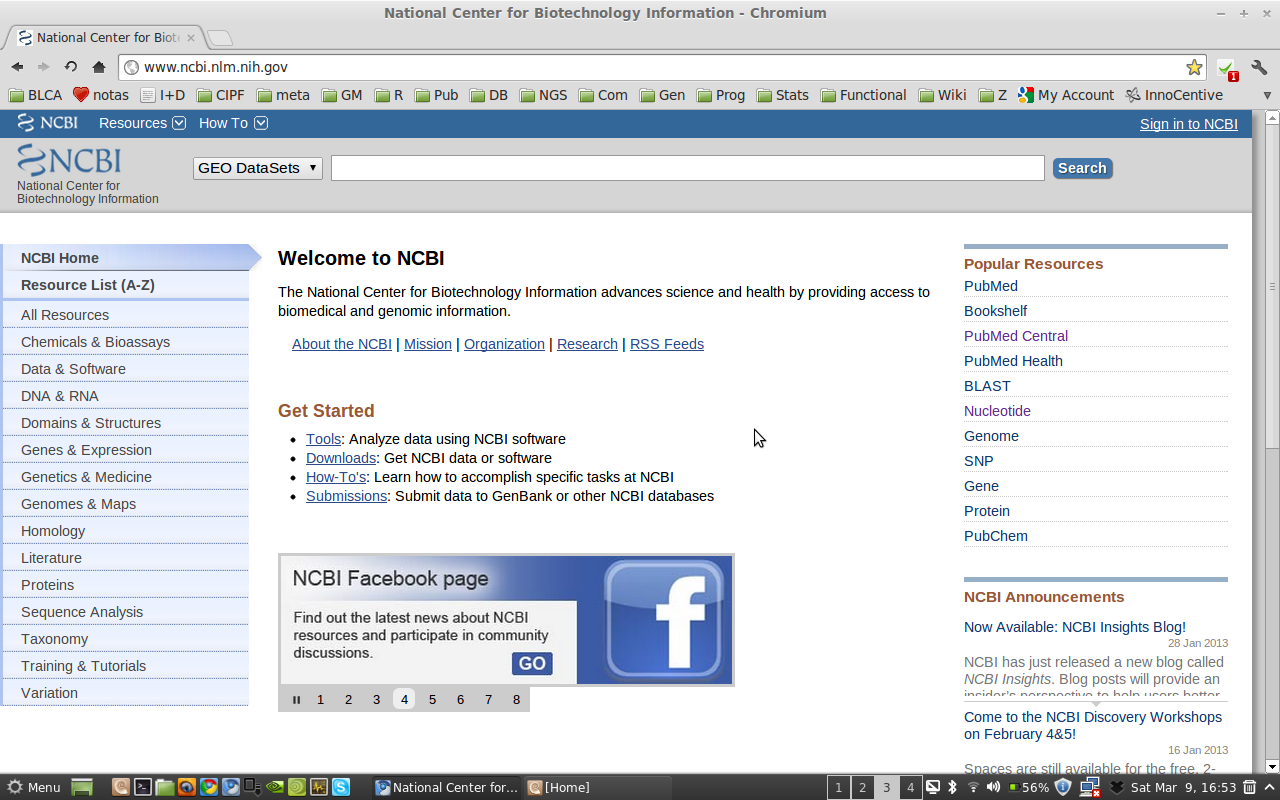
\includegraphics[width=\linewidth]{ncbi1}}
  \end{center}

\end{frame}

%%%%%%%%%%%%%%%%%%%%%%%%%%%%%%%%%%%%%%%%%%%%%%%%%%%%%%%%%%%%%%%%%%%%%%%%%%%%%%%%

\begin{frame}
  \frametitle{Usual searches}

  \begin{itemize}
  \item Search for a GEO accession \dots form a \href{http://www.plosone.org/article/info\%3Adoi\%2F10.1371\%2Fjournal.pone.0035915}{publication}.
  \item Search for example data for a particular platform 
  \item Keyword 
  \item Date \dots
  \end{itemize}

\end{frame}

%%%%%%%%%%%%%%%%%%%%%%%%%%%%%%%%%%%%%%%%%%%%%%%%%%%%%%%%%%%%%%%%%%%%%%%%%%%%%%%%

\begin{frame}
  \frametitle{Download GEO data}

  \begin{itemize}
  \item Links on Series records are provided at the foot of each GEO Series record web page.
    Ex. \href{http://www.ncbi.nlm.nih.gov/geo/query/acc.cgi?acc=GSE37761}{GSE37761 web}.
  \item FTP download: \url{ftp://ftp.ncbi.nlm.nih.gov/geo/}. 
    Ex. {\footnotesize \url{ftp://ftp.ncbi.nlm.nih.gov/geo/series/GSE37nnn/GSE37761/}}
  \item \href{http://www.ncbi.nlm.nih.gov/geo/info/geo_paccess.html}{Programmatic access to GEO}: 
    server-side programs to retrieve data; can be used with a fixed URL syntax.
  \end{itemize}

\end{frame}

%%%%%%%%%%%%%%%%%%%%%%%%%%%%%%%%%%%%%%%%%%%%%%%%%%%%%%%%%%%%%%%%%%%%%%%%%%%%%%%%

\begin{frame}[allowframebreaks]
  \frametitle{Series Data Formats}
  
  \begin{center}
    %\includegraphics[scale=0.3]{} 
    \href{http://www.ncbi.nlm.nih.gov/geo/query/acc.cgi?acc=GSE37761}{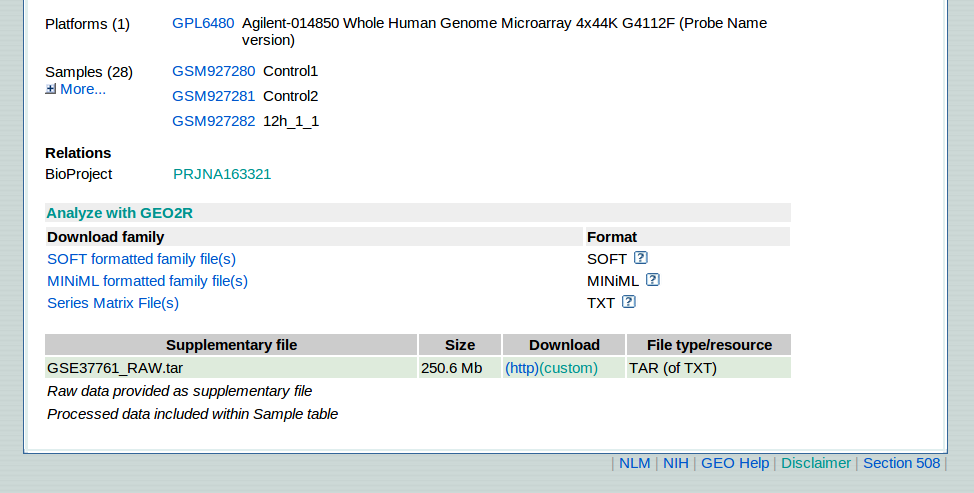
\includegraphics[width=\linewidth]{geo_download_data1}}
  \end{center}

  \framebreak

  \begin{itemize}
  \item SOFT formatted family file(s): complete data and metadata (gene information) in a single file.
  \item MINiML formatted family file(s): complete data and metadata in separated files.
  \item Series Matrix File(s): complete data in a tab delimited matrix; no metadata information.

    \bigskip

  \item Supplementary files: usually raw data.
  \end{itemize}

  \bigskip

  We generally use the \textit{Series Matrix} format and may be the \textit{platform} file within the \textit{MINiML} folder.

\end{frame}

%%%%%%%%%%%%%%%%%%%%%%%%%%%%%%%%%%%%%%%%%%%%%%%%%%%%%%%%%%%%%%%%%%%%%%%%%%%%%%%%

\begin{frame}
  \frametitle{GEO internal tools}

  GEO2R: simple analysis for GEO Series or DataSets

  \begin{center}
    %\includegraphics[scale=0.3]{} 
    \href{http://www.ncbi.nlm.nih.gov/geo/geo2r/?acc=GSE37761}{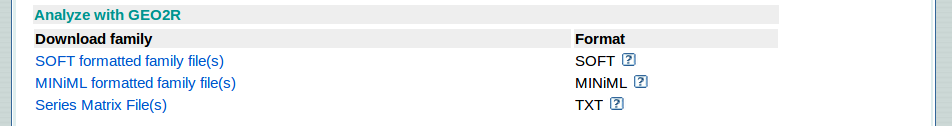
\includegraphics[width=\linewidth]{geo_tools2}}
  \end{center}

  \begin{itemize}
  \item explore \textit{Value distribution}: box-plot and summary statistics.
  \item explore single gene expression \textit{Profile graph}
  \item perform a differential expression analysis to compare two or more groups of Samples.
  \item clustering (just for DataSets)
  \end{itemize}

\end{frame}

%%%%%%%%%%%%%%%%%%%%%%%%%%%%%%%%%%%%%%%%%%%%%%%%%%%%%%%%%%%%%%%%%%%%%%%%%%%%%%%%

\begin{frame}
  \frametitle{Bioconductor Packages}
  
  \url{http://www.bioconductor.org/packages/release/}
  
  \bigskip
  
  \begin{itemize}
  \item GEOmetadb: A compilation of metadata from NCBI GEO.
  \item GEOsubmission: Prepares microarray data for GEO submission.
  \item GEOquery: \textbf{Get data} from NCBI Gene Expression Omnibus.
  \end{itemize}

\end{frame}


% %%%%%%%%%%%%%%%%%%%%%%%%%%%%%%%%%%%%%%%%%%%%%%%%%%%%%%%%%%%%%%%%%%%%%%%%%%%%%%%%
% %%%%%%%%%%%%%%%%%%%%%%%%%%%%%%%%%%%%%%%%%%%%%%%%%%%%%%%%%%%%%%%%%%%%%%%%%%%%%%%%

\begin{frame}
  \frametitle{References}

  \begin{itemize}
  \item \url{http://www.ncbi.nlm.nih.gov/geo/info/}
  \item \url{http://en.wikipedia.org/wiki/Microarray_databases}
  \item \url{http://en.wikipedia.org/wiki/MIAME}
  \end{itemize}

\end{frame}  

% %% FIN DOCUMENTO %%%%%%%%%%%%%%%%%%%%%%%%%%%%%%%%%%%%%%%%%%%%%%%%%%%%%%%%%%%%%%%
\end{document}

